% Beamer Presentation

\documentclass[13pt]{beamer}
\usetheme{metropolis}
\usepackage{eulervm}
\usepackage{appendixnumberbeamer}
\usepackage{amsmath}

\DeclareMathOperator{\Tr}{Tr}

\setsansfont[BoldFont={Fira Sans}]{Fira Sans Light}
\setmonofont{Fira Mono}
\metroset{block=fill}

\title{Mean-Field Study of Kondo Phase Diagram}
\date{\today}
\author{\textbf{Elis Roberts} - \textit{supervised by} Claudio Castelnovo \textit{\&} Garry Goldstein}
\institute{University of Cambridge}
\titlegraphic{\hfill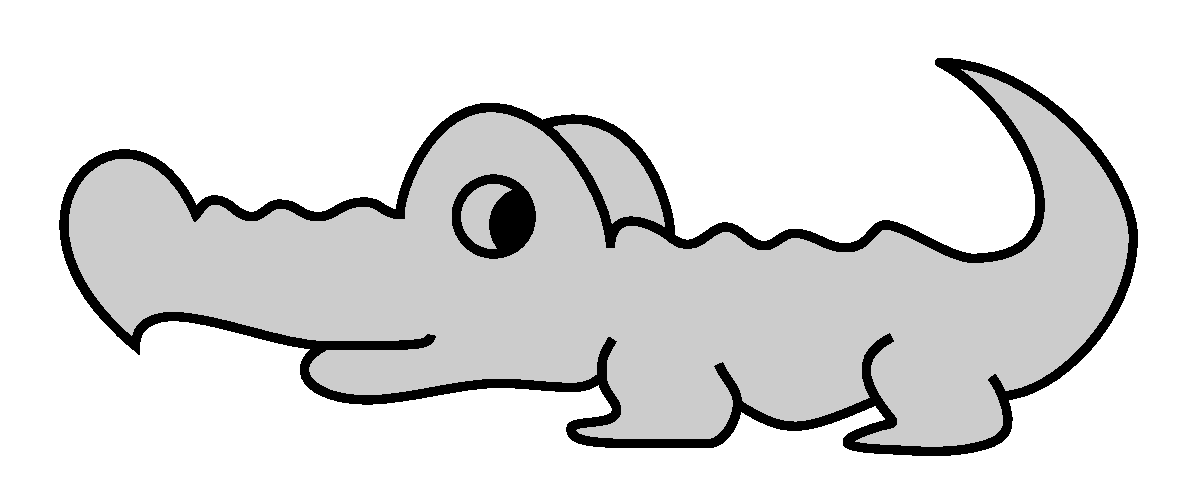
\includegraphics[height=1cm]{Figures/croc_dima.eps}}

\begin{document}
  \maketitle

  \begin{frame}{Plan}
  \setbeamertemplate{section in toc}[sections numbered]
  \tableofcontents[hideallsubsections]
  \end{frame}

  \section{Introduction}

  \begin{frame}{Kondo Model}
    Single localised spin interacting with conduction electrons $c^{}_{k,\sigma} $

    \vfill

    \begin{block}{Model Hamiltonian}
      $$ H_{\text{Kondo}}=\sum_{k,\sigma}\epsilon_{k} c_{k,\sigma}^{\dagger}c^{}_{k,\sigma}+J\vec{S}\cdot\vec{s}(0) $$
    \end{block}

    \begin{itemize}
    \item Can map impurity spin DOF to fermions $ f_{\sigma} $
    \item Think of it as describing interacting fermions $ c_{k,\sigma} $ and $ f_{\sigma} $

  \end{itemize}
    \vfill

    \begin{alertblock}{Goal}
      Describe phase diagram for this model using \emph{mean-field theory}
    \end{alertblock}

  \end{frame}

  \begin{frame}{Path Integral $ \rightarrow $ Mean-Field Theory}

  \begin{itemize}
    \item Project framed in terms of path integral
    \item Treats Boltzmann sum as a functional integral over field configurations
  \end{itemize}

    \begin{block}{Many-Body Path Integral}
      $$ Z = \Tr{e^{- \beta H}} = \int \mathcal{D} [c^\dagger, c]~e^{-\int_{0}^{\beta} \,d\tau~L} $$
    \end{block}

  \begin{itemize}
    \item Similar to Feynman path integral approach, but with \textit{imaginary time} $ \tau = i t / \hslash $ and associated Lagrangian $ L $
  \end{itemize}

  \begin{block}{Mean-Field Theory}
    Avoid this difficult integral by making stationary phase approximation \hfill i.e. \alert{\textit{minimise}}
  \end{block}

  \end{frame}

  \begin{frame}{New Fields}

  \begin{itemize}
    \item Lagrangian similar to original Hamiltonian, with extra dynamical terms: $ L = H_{\text{Kondo}} + c^\dagger \partial_\tau c$
    \item \textbf{But}, interaction introduces difficult non-quadratic terms

    \vfill

    \begin{alertblock}{Resolution} % Make W boson analogy
      Introduce a new field $ V $ that mediates this interaction:
      \begin{figure}
        \centering
        \includegraphics[width=0.95\textwidth]{Figures/V_field.png}
      \end{figure}
    \end{alertblock}
  \end{itemize}

  \end{frame}

  \begin{frame}{Constraints}

  \begin{itemize}
    \item Making such variable changes may require \textbf{constraints}
  

  \begin{exampleblock}{\textit{e.g.} Spin-1/2 $ \rightarrow $ Fermion Mapping}
  $$ s_z = \tfrac{1}{2} (f^{\dagger}_{\uparrow} f^{}_{\uparrow} - f^{\dagger}_{\downarrow} f^{}_{\downarrow}), \quad s_{+} = f^{\dagger}_{\uparrow} f^{}_{\downarrow}, \quad s_{-} = f^{\dagger}_{\downarrow} f^{}_{\uparrow} $$

  Unfaithful representation unless constraint imposed: $$ f^{\dagger}_{\uparrow} f^{}_{\uparrow} + f^{\dagger}_{\downarrow} f^{}_{\downarrow} = 1 $$
  \end{exampleblock}

    \item Implement constraints by adding Lagrange multipliers $ \{ \lambda_i \}$ and extremesing too: $$ L \quad = \quad \ldots \quad + \quad \lambda_{\text{RN}} (f^{\dagger}_{\uparrow} f^{}_{\uparrow} + f^{\dagger}_{\downarrow} f^{}_{\downarrow} - 1) $$

  \end{itemize}
  \end{frame}

  \begin{frame}{Soft-Constraint Approach}

  \begin{itemize}
    \item Now consider rewriting the same constraint: $$ (1 - n_{\uparrow} - n_{\downarrow})^2 = 0 $$
    \item Equivalent \textbf{but} can't be done at mean-field level since $$ \langle (1 - n_{\uparrow} - n_{\downarrow})^2 \rangle \neq 0 $$

    \end{itemize}

    \begin{block}{Soft-Constraint}
      How about introducing a new fermion $ h $ obeying $ h^{\dagger} h^{} = 0 $, but combining these constraints by instead imposing $$ (1 - n_{\uparrow} - n_{\downarrow})^2 - K h^{\dagger} h^{} = 0 \quad ? $$
    \end{block}

  \end{frame}

  \begin{frame}{Soft-Constraint Approach}

  \begin{itemize}
    \item How could $ (1 - n_{\uparrow} - n_{\downarrow})^2 - K h^{\dagger} h^{} = 0 $ be any better?
    \item Have introduced a new free parameter $ K $ into description
    \item Provided $ K > 0 $ and $ K \neq 1 $, constraint operator now has positive \textit{and} negative eigenvalues: $$ \{ \quad 1, \quad (1 - K), \quad 0, \quad -K \quad \} $$
  \end{itemize}

  \begin{block}{Consequence}
  New composite constraint picks out both constraints, while still being possible at mean-field level
  \end{block}
  \end{frame}

  \section{Finite Temperature Study}

  \begin{frame}{Solving Mean-Field Equations}

    \begin{block}{Obtaining MF Equations}
    Minimise free energy $ F_{\text{MF}} = - k_{\text{B}} T \ln{Z} $ wrt all variables: $$ \frac{\partial F_{\text{MF}}}{\partial \Delta} = 0, \qquad \frac{\partial F_{\text{MF}}}{\partial \lambda_{\text{SC}}} = 0, \qquad \ldots $$
    \end{block}

    \begin{itemize}
      \item Restricting search to reals leads to 9 equations
      \item Isotropy of $ B = 0 $ case $ \implies $ 7 unique variables / equations
    \end{itemize}

    \vfill

    \centering \alert{\Large How does this relate to a phase diagram?}
  \end{frame}

  \begin{frame}{Defining an Order Parameter $ \Delta $}

  \begin{itemize}
    \item Recall the (now constant) bosonic field $ V $ mediating the interaction

  \begin{block}{Now Define $ \Delta $}
  $$ \Delta \propto | V |^{2} $$
  \end{block}

    \item $ \Delta \rightarrow 0 $ implies $ c_{k, \sigma} $ and $ f_{\sigma} $ fermions no longer interact
    \item Value of $ \Delta $ characterises different phases
  \end{itemize}

  \end{frame}

  \begin{frame}{Expected Phase Diagram \textit{(Approximate)}}

  \begin{figure}
    \centering
    \includegraphics[width=0.75\textwidth]{Figures/phase_diagram.pdf}
  \end{figure}

  \end{frame}

  \begin{frame}{Classifying Phase Transitions}

  \begin{itemize}
    \item Phase transitions classified by discontinuities in successive derivatives of $ F $ wrt thermodynamic variables
  \end{itemize}

  \begin{alertblock}{Limitation of Mean-Field Theory}
    \begin{itemize}
      \item As usual, mean-field theory predicts a phase transition
      \item \textbf{But}, more advanced treatments show a smooth \emph{crossover}
    \end{itemize}
  \end{alertblock}

  \begin{itemize}
    \item Can study nature of PT by looking at form of $ F(T) $
  \end{itemize}

  \begin{exampleblock}{\textit{e.g.} Heat Capacity}
  $$ C = \frac{\partial E}{\partial T} = - T \frac{\partial^2 F}{\partial T^2} $$
  \end{exampleblock}

  \end{frame}

  \begin{frame}{Behaviour of Order Parameter $ \Delta $}

  \begin{figure}
    \centering
    \includegraphics[width=0.75\textwidth]{Figures/delta_vs_T.pdf}
  \end{figure}

  \end{frame}

  \begin{frame}{Unavoidable Phase Transition?}

  Crucially, $ \Delta < 0 $ unphysical $ \implies $ $ \Delta $ assumes \emph{piecewise} form

    \begin{itemize}
      \item \textbf{Q:} Can a piecewise function have all derivatives match?
      \item \textbf{A:} Not if it has a Taylor expansion.
    \end{itemize}

  \begin{exampleblock}{What about non-analytic functions?}
    $$ f(T) \approx 
    \begin{cases}
    e^{- 1 / (T - T_{\text{c}})^2} & T < T_{\text{c}} \\
    0 & T \geq T_{\text{c}}
    \end{cases} $$
  \end{exampleblock}

  Could we promote $ K \rightarrow K(T) $ to remove discontinuities in $ \partial^n F $?

  \end{frame}

  \begin{frame}{Unavoidable Phase Transition?}
    \begin{itemize}
      \item Can't seem to remove this phase transition
      \item $ K $ still limited by $ \langle (1 - n_{\uparrow} - n_{\downarrow})^2 \rangle \leq 1 $
      \item Choosing $ K(T) $ made complicated since $ \widetilde{K} = K \langle h^{\dagger} h \rangle $
      \item Have thermal occupation of $ h $ fermion too: $$ \langle h^{\dagger} h \rangle = \frac{1}{1 + e^{- \beta K \lambda_{\text{SC}}}} $$
    \end{itemize}

  \end{frame}

  \section{Conclusion}

  \begin{frame}{Take Home Points}

  \begin{itemize}
    \item Path integrals can describe many-body systems at finite $ T $
    \item MF theory considers optimal solution only - much easier
    \item Soft-Constraint is an alternative approach to implementing constraints in the Lagrangian
    \item SC introduces a new free parameter into description, but is seemingly not enough to remove second-order PT
  \end{itemize}

  \end{frame}

  \appendix

  \section{Backup}

  \begin{frame}{Final Lagrangian}
    \begin{align*}
    L \quad &= \sum_{k,\sigma} c^{\dagger}_{k,\sigma} \left( \frac{d}{\,d\tau} + \epsilon_k - \mu \right) c^{}_{k,\sigma} + \sum_{\sigma} f^{\dagger}_{\sigma} \frac{d}{\,d\tau} f^{}_{\sigma} + h^{\dagger} \frac{d}{\,d\tau}h \\
    &+ e^{\dagger} \frac{d}{\,d\tau} e  + \sum_{\sigma} p^{\dagger}_{\sigma} \frac{d}{\,d\tau} p^{}_{\sigma} + d^{\dagger} \frac{d}{\,d\tau} d \\
    &+ \sum_{\sigma} \lambda^{}_{\sigma} (f^{\dagger}_{\sigma} f^{}_{\sigma} - p^{\dagger}_{\sigma} p^{}_{\sigma} - d^{\dagger} d^{} ) \\
    &+ \lambda_{\text{KR}} ( e^{\dagger} e + \sum_{\sigma} p^{\dagger}_{\sigma} p^{}_{\sigma} + d^{\dagger} d - 1 ) + \lambda_{\text{SC}} ( e^{\dagger} e + d^{\dagger} d - K h^{\dagger} h) \\
    &+ 2 \frac{V V^{\ast}}{J} + \sum_{k,\sigma} \left( V^{\ast} c^{\dagger}_{k,\sigma} z^{}_{\sigma} f^{}_{\sigma} + V f^{\dagger}_{\sigma} z^{\dagger}_{\sigma} c^{}_{k,\sigma} \right)
    \end{align*}
  \end{frame}

\end{document}